\documentclass{beamer}

\usetheme{simple}

\newcommand{\emojiskull}{\includegraphics[width=12pt]{img/skull.png}}

\usepackage{caption}
\usepackage{xcolor}
\usepackage{fancyvrb, hyperref}
\usepackage{ulem}
\usepackage{subcaption}
\usetikzlibrary{positioning,calc,automata}

\title{CSC363 Tutorial \#7}
\subtitle{Hamiltonian Path Problem}
\date{March 9, 2022}
\institute{}

\newcommand{\N}{{\mathbb N}}
\newcommand{\R}{{\mathbb R}}
\newcommand{\inner}[1]{\langle #1 \rangle}

\setwatermark{\includegraphics[height=8cm]{img/chungus.png}}

\begin{document}

\maketitle

\begin{frame}{Learning objectives this tutorial}
\begin{itemize}
\item Formulate the \textit{Hamiltonian Cycle Problem}, and then the \textit{Hamiltonian Path Problem}.
\item Show that the \textit{Hamiltonian Cycle Problem} (and the Hamiltonian Path Problem) can be decided by a NTM in poly-time.
\item Show that the \textit{Hamiltonian Cycle Problem} (and the Hamiltonian Path Problem) can be \textit{verified} in poly-time.
\end{itemize}
\end{frame}

\begin{frame}{Some Clarifications}
\begin{itemize}
\item When we say that a TM $M$ runs in $f(n)$-time, we mean the following:

\textit{For all inputs of length $n$ (in terms of number of characters), the computation $M(n)$ halts within $f(n)$ steps.}

\item When we say that a language $L$ is decidable in $f(n)$-time, we mean that \textit{there is some TM that decides $L$ in $f(n)$-time.}
\end{itemize}
\end{frame}

\begin{frame}{Hamilton}
\textbf{Question:} Who's this person?

\begin{figure}[h]
    \centering
    \includegraphics[width=8cm]{img/hamilton.jpg}
\end{figure}

\pause

\textbf{Ans:} Sir William Rowan Hamilton, LL.D, DCL, MRIA, FRAS.

\end{frame}

\begin{frame}{Hamilton Lore}

\begin{figure}[h]
    \centering
    \includegraphics[width=3cm]{img/hamilton.jpg}
\end{figure}

List of things attributed to \textit{Sir William Rowan Hamilton, LL.D, DCL, MRIA, FRAS}:
\pause
\begin{itemize}
    \item Quaternions. (Think complex numbers $a + bi$ with $i^2 = -1$ aren't enough? Introducing 4-dimensional numbers $a + bi + cj + dk$ with $i^2 = j^2 = k^2 = ijk = -1$!)
    \pause
    \item Physics, specifically \textit{Hamiltonian Mechanics}. {\tiny{i dont know what this is}}
    \item Astronomy. {\tiny{i dont know astronomy either}}
    \item Some graph theory.
    \item Other uninteresting stuff
\end{itemize}

\end{frame}

\begin{frame}{Hamilton Lore}

\begin{figure}[h]
    \centering
    \includegraphics[width=9cm]{img/quaternion_plaque.jpg}
    \caption*{Around Broom Bridge, Dublin. Vandalized many times, of course.}
\end{figure}

There's also a \textit{Hamilton Walk} event that takes place every year from Dunsink Observatory in Dublin Broom Bridge. Would be funny if they walked in a \textit{Hamiltonian path}, eh.

\end{frame}

\begin{frame}{Hamilton}
\textbf{Question:} What would someone, living in 19th century Ireland, do when they were bored?

\pause

\textbf{Ans:} Math.\footnote{Not sure about other 19th century Irishpeople, but Hamilton certainly did.}  \pause More specifically, think about whether they can ``walk'' across a dodecahedron in a loop, visiting every vertex once.

\begin{figure}[h]
    \centering
    \includegraphics[width=1.5cm]{img/Dodecahedron.png}
\end{figure}

\pause
 
Let's try it! Here's the dodecahedron projected to 2D space. \pause

\textbf{Task:} Can you find a cycle in the graph below that visits every vertex exactly once?

\begin{figure}[h]
    \centering
    \includegraphics[width=3cm]{img/projected_dodecahedron.png}
\end{figure}

\end{frame}

\begin{frame}{Hamilton}
\textbf{Task:} Can you find a cycle in the graph below that visits every vertex exactly once?

\begin{figure}[h]
    \centering
    \includegraphics[width=3cm]{img/projected_dodecahedron.png}
\end{figure}

\pause

\textbf{Ans:} Yes!

\begin{figure}[h]
    \centering
    \includegraphics[width=3cm]{img/projected_dodecahedron_path.png}
    \caption*{\small{This kinda reminds me of ``connect the dots'' games I used to play as a kid}}
\end{figure}

\end{frame}

\begin{frame}{Hamiltonian Cycle Problem}

The previous ``connect the dots in a loop'' game is a specific instance of the \textbf{Hamiltonian Cycle Problem}. 

\pause


In the Hamiltonian Cycle Problem, you are given a graph (undirected in our context), and asked to determine whether a \textit{Hamiltonian Cycle} exists.

\pause \vspace{2mm}

\textbf{Definition:} Given a graph $G = (V, E)$, a \textbf{Hamiltonian Cycle} is a cycle that contains each vertex $v \in V$ exactly once. 

\pause \vspace{2mm}

\textbf{Task:} Determine whether Hamiltonian cycles exist in the following graphs.

\begin{figure}
    \centering
    \begin{subfigure}{0.3\textwidth}
    \centering
    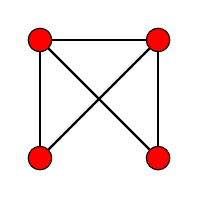
\begin{tikzpicture}[vertex/.style={circle,draw,minimum size=1mm, fill=red, inner sep=3pt]}]
        \node[vertex] (v1) at (0, 0) {};
        \node[vertex] (v2) at (1.5, 0) {};
        \node[vertex] (v3) at (0, 1.5) {};
        \node[vertex] (v4) at (1.5, 1.5) {};
        \draw[thick] (v2) -- (v3);
        \draw[thick] (v1) -- (v4);
        \draw[thick] (v2) -- (v4);
        \draw[thick] (v3) -- (v4);
        \draw[thick] (v1) -- (v3);
    \end{tikzpicture}
    \end{subfigure}
    \begin{subfigure}{0.3\textwidth}
    \centering
    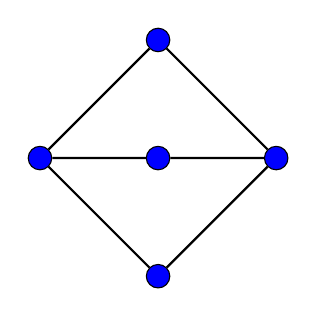
\begin{tikzpicture}[vertex/.style={circle,draw,minimum size=1mm, fill=blue, inner sep=3pt]}]
        \node[vertex] (v1) at (0, 0) {};
        \node[vertex] (v2) at (1.5, 0) {};
        \node[vertex] (v3) at (3, 0) {};
        \node[vertex] (v4) at (1.5, 1.5) {};
        \node[vertex] (v5) at (1.5, -1.5) {};
        \draw[thick] (v1) -- (v2) -- (v3) -- (v4) -- (v1) -- (v5) -- (v3);
    \end{tikzpicture}
    \end{subfigure}
    \begin{subfigure}{0.3\textwidth}
    \centering
    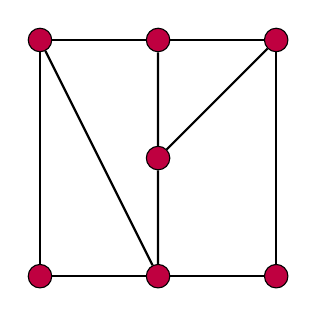
\begin{tikzpicture}[vertex/.style={circle,draw,minimum size=1mm, fill=purple, inner sep=3pt]}]
        \node[vertex] (v1) at (0, 0) {};
        \node[vertex] (v2) at (1.5, 0) {};
        \node[vertex] (v3) at (3, 0) {};
        \node[vertex] (v6) at (0, 3) {};
        \node[vertex] (v5) at (1.5, 3) {};
        \node[vertex] (v4) at (3, 3) {};
        \node[vertex] (v7) at (1.5, 1.5) {};
        \draw[thick] (v1) -- (v2) -- (v3) -- (v4) -- (v5) -- (v6) -- (v1);
        \draw[thick] (v6) -- (v2) -- (v7) -- (v5);
        \draw[thick] (v7) -- (v4);
    \end{tikzpicture}
    \end{subfigure}
\end{figure}

\end{frame}


\begin{frame}{Hamiltonian Cycle Problem}
\textbf{Ans:} The left and right graphs have Hamiltonian cycles, while the middle graph doesn't.

\begin{figure}
    \centering
    \begin{subfigure}{0.3\textwidth}
    \centering
    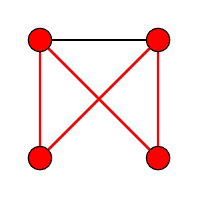
\begin{tikzpicture}[vertex/.style={circle,draw,minimum size=1mm, fill=red, inner sep=3pt]}]
        \node[vertex] (v1) at (0, 0) {};
        \node[vertex] (v2) at (1.5, 0) {};
        \node[vertex] (v3) at (0, 1.5) {};
        \node[vertex] (v4) at (1.5, 1.5) {};
        \draw[thick] (v2) -- (v3);
        \draw[thick] (v1) -- (v4);
        \draw[thick] (v2) -- (v4);
        \draw[thick] (v3) -- (v4);
        \draw[thick] (v1) -- (v3);
        \draw[thick, red] (v1) -- (v4) -- (v2) -- (v3) -- (v1);
    \end{tikzpicture}
    \end{subfigure}
    \begin{subfigure}{0.3\textwidth}
    \centering
    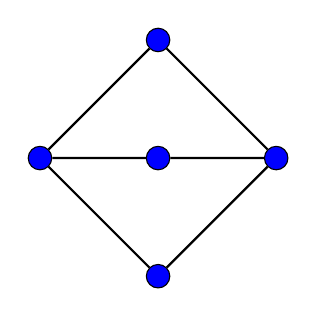
\begin{tikzpicture}[vertex/.style={circle,draw,minimum size=1mm, fill=blue, inner sep=3pt]}]
        \node[vertex] (v1) at (0, 0) {};
        \node[vertex] (v2) at (1.5, 0) {};
        \node[vertex] (v3) at (3, 0) {};
        \node[vertex] (v4) at (1.5, 1.5) {};
        \node[vertex] (v5) at (1.5, -1.5) {};
        \draw[thick] (v1) -- (v2) -- (v3) -- (v4) -- (v1) -- (v5) -- (v3);
    \end{tikzpicture}
    \end{subfigure}
    \begin{subfigure}{0.3\textwidth}
    \centering
    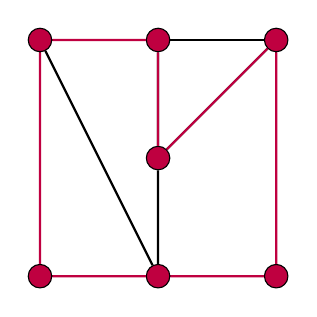
\begin{tikzpicture}[vertex/.style={circle,draw,minimum size=1mm, fill=purple, inner sep=3pt]}]
        \node[vertex] (v1) at (0, 0) {};
        \node[vertex] (v2) at (1.5, 0) {};
        \node[vertex] (v3) at (3, 0) {};
        \node[vertex] (v6) at (0, 3) {};
        \node[vertex] (v5) at (1.5, 3) {};
        \node[vertex] (v4) at (3, 3) {};
        \node[vertex] (v7) at (1.5, 1.5) {};
        \draw[thick] (v1) -- (v2) -- (v3) -- (v4) -- (v5) -- (v6) -- (v1);
        \draw[thick] (v6) -- (v2) -- (v7) -- (v5);
        \draw[thick] (v7) -- (v4);
        \draw[thick, purple] (v1) -- (v2) -- (v3) -- (v4) -- (v7) -- (v5) -- (v6) -- (v1);
    \end{tikzpicture}
    \end{subfigure}
\end{figure}


\pause

\textbf{Question:} How do we know that there is no Hamiltonian cycle for the middle graph?

\pause

\textbf{Ans:} \emojiskull brute force.

\pause

\textbf{Insight:} This gives us another ``hard to solve, easy to verify'' problem.

\end{frame}

\begin{frame}[fragile]{Hamiltonian Cycle Problem}
\textbf{Task:} Describe, in pseudocode, how you can ``brute-force'' the Hamiltonian cycle problem. What is the runtime?

\pause

\textbf{Ans:}
\begin{verbatim}
def has_hcycle(V, E):
  suppose V = {v1, v2, ..., vn}
  for every permutation {vi1, vi2, ..., vin} 
    of {v1, v2, ..., vn}:
    if vi1->vi2->...->vin->vi1 is a valid path in the graph:
      return True
  return False
\end{verbatim}

The runtime is... \pause $O(n! m)$ (since there are $n!$ many permutations of $n$ vertices, and checking each permutation takes $O(m)$).
\pause

\textbf{Question:} Can we do better?

\textbf{Ans:} \emojiskull we don't know... (this is akin to solving the P vs NP problem)\footnote{The Hamiltonian Cycle problem is \textit{NP-complete}.}

\end{frame}

\begin{frame}{Hamiltonian Cycle Problem}

The runtime is... $O(n! m)$ (since there are $n!$ many permutations of $n$ vertices, and checking each permutation takes $O(m)$).

\begin{figure}
    \centering
    \includegraphics[width=8cm]{img/factorial_time.png}
    \caption*{\color{blue}\href{https://www.reddit.com/r/ProgrammerHumor/comments/n8bgw1/boss_makes_a_dollar_i_make_a_dime/}{source}}
\end{figure}

\end{frame}


\begin{frame}{Hamiltonian Cycle Problem}

There's a similar problem, called the \textbf{Hamiltonian Path Problem}, which involves visiting every vertex exactly once in a path (without having to loop back to the beginning).

\begin{figure}
    \centering
    \begin{subfigure}{0.3\textwidth}
    \centering
    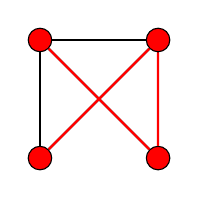
\begin{tikzpicture}[vertex/.style={circle,draw,minimum size=1mm, fill=red, inner sep=3pt]}]
        \node[vertex] (v1) at (0, 0) {};
        \node[vertex] (v2) at (1.5, 0) {};
        \node[vertex] (v3) at (0, 1.5) {};
        \node[vertex] (v4) at (1.5, 1.5) {};
        \draw[thick] (v2) -- (v3);
        \draw[thick] (v1) -- (v4);
        \draw[thick] (v2) -- (v4);
        \draw[thick] (v3) -- (v4);
        \draw[thick] (v1) -- (v3);
        \draw[thick, red] (v1) -- (v4) -- (v2) -- (v3);
    \end{tikzpicture}
    \end{subfigure}
    \begin{subfigure}{0.3\textwidth}
    \centering
    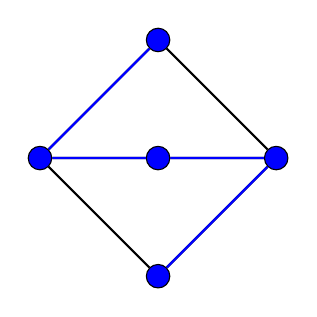
\begin{tikzpicture}[vertex/.style={circle,draw,minimum size=1mm, fill=blue, inner sep=3pt]}]
        \node[vertex] (v1) at (0, 0) {};
        \node[vertex] (v2) at (1.5, 0) {};
        \node[vertex] (v3) at (3, 0) {};
        \node[vertex] (v4) at (1.5, 1.5) {};
        \node[vertex] (v5) at (1.5, -1.5) {};
        \draw[thick] (v1) -- (v2) -- (v3) -- (v4) -- (v1) -- (v5) -- (v3);
        \draw[thick, blue] (v4) -- (v1) -- (v2) -- (v3) -- (v5);
    \end{tikzpicture}
    \end{subfigure}
    \begin{subfigure}{0.3\textwidth}
    \centering
    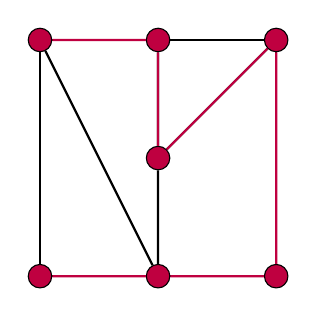
\begin{tikzpicture}[vertex/.style={circle,draw,minimum size=1mm, fill=purple, inner sep=3pt]}]
        \node[vertex] (v1) at (0, 0) {};
        \node[vertex] (v2) at (1.5, 0) {};
        \node[vertex] (v3) at (3, 0) {};
        \node[vertex] (v6) at (0, 3) {};
        \node[vertex] (v5) at (1.5, 3) {};
        \node[vertex] (v4) at (3, 3) {};
        \node[vertex] (v7) at (1.5, 1.5) {};
        \draw[thick] (v1) -- (v2) -- (v3) -- (v4) -- (v5) -- (v6) -- (v1);
        \draw[thick] (v6) -- (v2) -- (v7) -- (v5);
        \draw[thick] (v7) -- (v4);
        \draw[thick, purple] (v1) -- (v2) -- (v3) -- (v4) -- (v7) -- (v5) -- (v6);
    \end{tikzpicture}
    \end{subfigure}
    \caption*{The middle graph has a solution to the Hamiltonian Path Problem.}
\end{figure}

\end{frame}

\begin{frame}[fragile]{NTM solution to Hamiltonian Cycle Problem}

\textbf{Task:} Build a poly-time NTM that decides the language
$$\mathrm{HC} = \{G: \text{There is a Hamiltonian Cycle in $G$}\}.$$

You should define \verb|in_HC(V, E)| (where $(V, E)$ is the graph).

\pause

\textbf{Ans:}
\begin{verbatim}
in_HC(V, E):
  choose a permutation (v1, ..., vn) of V # nondeterministic!
  for i in 1, ..., n-1:
    if (vi, v(i+1)) not in E:
      reject
  if (vn, v1) not in E:
    reject
  accept
\end{verbatim}

\end{frame}

\begin{frame}[fragile]{NTM solution to Hamiltonian Cycle Problem}

\textbf{Task:} Build a poly-time TM \verb|verify_HC(V, E, s)| such that
\begin{align*}
    (V, E) \in \mathrm{HC} \Leftrightarrow &\text{There is some input s such that}\\
    &\text{\texttt{verify\_HC(V, E, s)} accepts}.
\end{align*}

\pause
\vspace{-3mm}
\textbf{Ans:}
\vspace{-3mm}
\begin{verbatim}
verify_HC(V, E, s: string):
  let V = (v1, ..., vn)
  if s is not of the form "(v{k1}, ..., v{kn}})":
    reject
  parse s to extract vertices vk1, ..., vkn
  for i in range(n-1):
    if (vki, vk(i+1)) not in E:
      reject
  if (vkn, vk1) not in E:
    reject
  accept
\end{verbatim}

\pause

\verb|verify_HC(V, E, s)| acts as a \textit{verifier}: it checks whether a prospective ``solution'' \verb|s| to the Hamiltonian Cycle problem actually works.

\end{frame}

\begin{frame}[fragile]{NTM poly-time versus verifiable in poly-time}

There is a more general definition of a \textit{verifier}.

\vspace{2mm}

\textbf{Definition:} A verifier $V$ for a language $L$ is a Turing machine that satisfies
$$x \in L \Leftrightarrow (\exists s) \text{V(x, s) accepts}.$$

A string $s$ is called a \textbf{certificate} if $V(x, s)$ accepts.\\
\end{frame}








\end{document}